\documentclass[12pt]{report}
\title{Mid Term Project}
\usepackage{amsmath}
%\usepackage{maplestd2e}
\usepackage{tikz}
\usetikzlibrary{arrows.meta,shapes.misc,patterns,shapes.symbols,decorations.pathreplacing,decorations}
\usepackage{amssymb}
\AtBeginDocument{\renewcommand{\chaptername}{}}
\usepackage{microtype}
\usepackage[bottom=30 mm, top=25 mm, left=25 mm, right=25 mm]{geometry}
\usepackage{multicol}
\usepackage{titlesec} 
\usepackage{graphicx}
\usepackage{listings}
\usepackage{xcolor}
\usepackage{amsmath}
\usepackage{subfigure}
\usepackage{subfig}
\usepackage{wasysym}
\usepackage{wrapfig}
\usepackage{float}
\usepackage{lipsum} 
\lstset{
    breaklines=true,
    tabsize=3,
    showstringspaces=false
}

\lstdefinestyle{Common}
{
    extendedchars=\true,
    language={[Visual]Basic},
    frame=single,
    framesep=3pt,
    framerule=0.4pt,
    xleftmargin=3.4pt,
    xrightmargin=3.4pt,
    rulecolor=\color{red}
}

\lstdefinestyle{A}
{
    style=Common,
    backgroundcolor=\color{yellow!10},
    basicstyle=\scriptsize\color{black}\ttfamily,
    keywordstyle=\color{orange},
    identifierstyle=\color{black},
    stringstyle=\color{red},
    commentstyle=\color{green}
}

\makeatletter 
\renewcommand\chapter{\thispagestyle{plain}%
\global\@topnum\z@
\@afterindentfalse
\secdef\@chapter\@schapter}
\makeatother 

\titleformat{\chapter}{\bfseries\Huge}{\thechapter.\quad}{0em}{}


\usepackage[utf8]{inputenc}
\parindent0pt

\begin{document}

%\setlength{\parindent}{3ex} 

\begin{large}

\thispagestyle{empty}
\begin{center}
\begin{figure}[t]
\centering
%
\includegraphics[scale=0.52]{sdsu_logo.png}
\end{figure}
\end{center}
\begin{center}
\Large{Department of Mathematics and Statistics}
\end{center}
\begin{center}
\Large{Prof. Joseph Mahaffy}
\end{center}
\begin{center}
\Large{Math 636, Mathematical Modeling}
\end{center}
\begin{verbatim}



\end{verbatim}
\begin{center}
\textbf{\Huge{Homework Assignment}}
\end{center}
\begin{verbatim}


\end{verbatim}
\rule{16,5 cm}{0.4pt}\\
\begin{center}
\textbf{\LARGE{Monte Carlo Methods}}\\[0,7 cm]
\end{center}
\rule{16,5 cm}{0.4pt}
\begin{verbatim}


\end{verbatim}

\begin{center}
 \textbf{by Matteo Polimeno} \\ 
\textbf{11/22/2017}\\

\end{center}
\end{large}


\newpage

\tableofcontents
\newpage

\sloppy

\newpage


\chapter{Problem 1}
\section{Part a}

We perform two Monte Carlo simulations for the Schmitz and Kwak study of the Deaconesse Hospital, using the following assumptions:\\
1) The daily case load is assumed to be fixed at 32 cases.\\
2) Random numbers are generated independently for each day.\\
3) All ENT, urology, and ophthalmology cases last 0.5 hours.\\
4) Half the urology cases and all ophthalmology cases do not go to the recovery room.\\
5) All ENT and the other half of urology cases go to the recovery room and are assumed to stay for 1.5 hours.\\
6) Any operation over 0.5 hours is considered major and requires 3 hours in the recovery room.\\
7) Surgery begins at 7:30 AM.\\
8) Preparation time is 0.25 hours in the operating room.\\
9) It takes 0.08 hours to transport patients from operating room to the recovery room.\\
10) It takes 0.25 hours to prepare the recovery room for the next occupant.\\
11) Operating rooms are used continuously as need arises with the first one vacated being the first one used.\\
12) The first vacated recovery bed is the first one filled as needed.\\
13) If no bed is available in the recovery room, then a new one is created.\\

Moreover, the simulation is run twice with 4 Operating Rooms and twice with 5 Operating Rooms.
The 32 cases scheduled for the day are assigned 32 random numbers.
The random numbers decide the type of surgery, which in turn determines how long the patient has surgery and if the patient goes to the recovery room and for how long.
The surgeries start at 7:30 AM filling the 4(5) operating rooms. Immediately after surgery each patient is transported, and the operating room is cleared for the next patient waiting.
The rules are followed until all 32 patients are seen, and the operating rooms and ICU beds are cleared.\\
We are asked to find the latest times at which the operating rooms and the recovery rooms are open in both scenarios.\\
We start by finding those times for the two 4-operating-rooms simulations. We call $MCMC_{4_{I}}$ the first simulation and $MCMC_{4_{II}}$ the second simulation respectively. For the latest times that the operating rooms are open, we get
$$
MCMC_{4_{I}} = 17.75
$$
$$
MCMC_{4_{II}} = 19.75,
$$
which means that in the two simulations with 4 operating rooms available, in the first case said rooms are open until 5:45PM, whereas in the second simulation, the operating rooms are open until 7:45PM.\\
This means that in the first simulation, since we assumed that surgery begins at 7:30AM, which is then the time at which operating rooms are first open, the operating rooms stay open for 10 hours and 15 minutes. In the second simulation, the operating rooms stay open for 12 hours and 15 minutes.\\
Therefore the average length of time that the 4 operating rooms are open each day for our two simulations is
$$
MCMC_{4_{Avg.t - I}} = 10.0625hrs
$$
$$
MCMC_{4_{Avg.t - II}} = 10.25hrs,
$$
which are, respectively, 10 hours and roughly 4 minutes, and 10 hours and 15 minutes.\\ 
Given these long periods, this is a first indication that 4-operating rooms might not be an optimised value to properly and promptly run operations in the hospital.\\
As for the latest time at which the recovery rooms are open, we get
$$
MCMC_{4_{Recovery-I}} = 20.83
$$
$$
MCMC_{4_{Recovery-II}} = 22.83,
$$
which means that in the first case the recovery rooms stay open until 8:55PM ca., whereas in the second simulation they close at 10:55PM ca.\\

Now, we list the results found for the two 5-operating-rooms simulations. For the latest time at which the operating rooms are open, we have
$$
MCMC_{5_{I}} = 16.25
$$
$$
MCMC_{5_{II}} = 18.25,
$$
which means that, in the first simulation operating rooms stay open until 4:15PM, whereas in the second one they stay open until 6:15PM. So in the first simulation, operating rooms stay open for 8 hours and 45 minutes (again, opening time is 7:30AM), whereas in the second simulation the operating rooms stay open for 10 hours 45 minutes.\\
Therefore the average length of time that the 5 operating rooms stay open for these two simulations is
$$
MCMC_{5_{Avg.t - I}} = 8.35hrs
$$
$$
MCMC_{5_{Avg.t - II}} = 8.40hrs,
$$
which are, respectively, 8 hours and 21 minutes and 8 hours and 24 minutes.\\
Confronting the average lengths of time that the operating rooms stayed open for the two simulations with the 4 operating rooms and the 5 operating rooms, our simulations seem to suggest that having 5 operating rooms available to perform daily surgeries seems to be a more efficient way to run operations at the hospital, as all 32 patients were taken care of, with regard to surgery, in less time.\\
Now for the latest times at which recovery rooms were open, we find
$$
MCMC_{5_{Recovery-I}} = 19.33
$$
$$
MCMC_{5_{Recovery-II}} = 21.33,
$$
which means that for the first simulation, the recovery rooms stay open until 7:20PM ca., whereas for the second simulation, the operating rooms stay open until 9:20PM ca.\\
Again, this seems to indicate that using 5 operating rooms would reduce the overall staying of each patient (surgery plus recovery), thus guaranteeing a more efficient way to run the hospital.

\section{Part b}
We assume that the recovery room must be staffed at all times by at least two nurses and that each nurse can handle at most 3 patients. Also, each nurse can only work an integer number of hours.\\
Then, according to our simulations, the number of nursing hours required to staff the recovery room is found to be
$$
MCMC_{4_{Nursing hrs-I}} = 39
$$
$$
MCMC_{4_{Nursing hrs-II}} = 39,
$$
for the two 4-operating-rooms simulations.\\
Whereas, for the two simulations with 5 operating rooms, we have
 $$
MCMC_{5_{Nursing hrs-I}} = 38
$$
$$
MCMC_{5_{Nursing hrs-II}} = 40.
$$

\section{Part c}
For this section, we are asked to run the simulations for 4 and 5 operating rooms 100 times and to provide  the mean longest time for both the operating and recovery rooms, mean average time of operating rooms being used, and the mean number of hours that are needed
for the nursing staff in the recovery room. Also, we are asked to compute the standard deviation (variance) of all of this information.\\
Attached to this page there is the Matlab code built to solve this problem.\\

\begin{tabular}{ |p{3cm}||p{3cm}|p{3cm}|p{3cm}|  }
 \hline
 \multicolumn{4}{|c|}{4 Operating Rooms MCMC - Computed Values} \\
 \hline
 Mean Time Op. Room Used&Mean Time Rec. Room Used&Mean Avg. Op. Room Used&Nursing Hours\\
 \hline
 17.4150  & 20.4800 & 8.8350 &   38.5900\\
 \hline
 \end{tabular}\\
 
 For these values, we compute the respective standard deviations to be
 \vspace{0.1mm}
 
  \begin{tabular}{ |p{3cm}||p{3cm}|p{3cm}|p{3cm}|  }
  \hline
  \multicolumn{4}{|c|}{4 Operating Rooms MCMC - Standard Deviations} \\
   \hline
 $\sigma$ for Mean Time Op. Room Used&$\sigma$ for Mean Time Rec. Room Used&$\sigma$ for Mean Avg. Op. Room Used&$\sigma$ for Nursing Hours\\
 \hline
 1.3148&  1.3276 & 0.9425 &4.6059\\
 \hline
\end{tabular}\\

\vspace{2mm}
Now we do the same for the 5-operating-rooms simulations and we obtain

\begin{tabular}{ |p{3cm}||p{3cm}|p{3cm}|p{3cm}|  }
 \hline
 \multicolumn{4}{|c|}{5 Operating Rooms MCMC - Computed Values} \\
 \hline
 Mean Time Op. Room Used&Mean Time Rec. Room Used&Mean Avg. Op. Room Used&Nursing Hours\\
 \hline
 15.9900  & 19.0575 & 7.2775 &   39.5300\\
 \hline
 \end{tabular}\\
 
 For these values, we compute the respective standard deviations to be
 \vspace{0.1mm}
 
  \begin{tabular}{ |p{3cm}||p{3cm}|p{3cm}|p{3cm}|  }
  \hline
  \multicolumn{4}{|c|}{5 Operating Rooms MCMC - Standard Deviations} \\
  \hline
 $\sigma$ for Mean Time Op. Room Used&$\sigma$ for Mean Time Rec. Room Used&$\sigma$ for Mean Avg. Op. Room Used&$\sigma$ for Nursing Hours\\
 \hline
 1.1907&  1.2113& 0.7757 &5.0681\\
 \hline
\end{tabular}

\chapter{Problem 2}
\section{Part a}
We have a Malthusian growth model with a 4\% annual growth, which is given by
$$
P_{n+1} = 1.04P_{n}, \quad P_{0}= 50,
$$
where $n$ is in years.\\
We want to find the population at $n=10$. This can be easily solved analytically by using the explicit expression
$$
P_{n} = 1.04^{n}P_{0},
$$
where $P_{0} = 50$.
Thus, for $n=10$, we get
$$
P_{10}=1.04^{(10)}(50)=74.0122
$$
Now, to find the time at which the population doubles, we simply solve
$$
1.04^{n}P_{0}=2P_{0},
$$
which yields
$$
n = \frac{\log2}{\log1.04} \approx 17.67,
$$
which means that the population will double after roughly seventeen years and eight months.\\

\section{Part b}
Starting with a population of 50 individuals at $t=0$, i.e. $P_{0}=50$, and giving each individual a 4\% chance of producing offspring each year, we consider a birth-only model for said population and run a Monte Carlo simulation for 10 years. As we know what $P_{0}$ is already, we will list the populations from $t=1$ to $t=10$, $(P_{1},...,P_{10})$, which are found to be
$$
P = (50, 52, 53, 59, 64, 68, 70, 72, 74, 78).
$$
Thus, for this simulation, we see that there is no offspring produced going from $P_{0}$ to $P_{1}$, but then our expected value for $P_{10}$ is 78, which is rougly 5\% greater than our expected value of 74.0310 computed analytically in Part a.

\section{Part c}
Now we run the simulation of Part b 1000 times and we provide the average population at 10 years and its standard deviation.
For $(P_{1},...,P_{10})$, we get
$$
P =(51.9570, 53.9890, 56.1420, 58.3660, 60.7440, 63.1640, 65.7250, 68.3320, 71.0770, 74.0310),
$$
with standard deviation $\sigma$ of
$$
\sigma = (1.3744, 1.9740, 2.4968, 2.9865, 3.5226, 3.9297, 4.3937, 4.8182, 5.3111, 5.7645)
$$
So, in Part a, we found our expected population after ten years to be $P_{10} = 74.0122$,
and after one thousand simulations we have found a mean value of $P_{10}=74.0310$, which is indeed very close to the expected value (in fact 0.25\permil\quad greater). However, if we take a look at the standard deviation for $n=10$, then we see that in the different simulation paths we have quite different values as we can notice by looking at $\sigma_{10}=5.7645$.\\ Moreover, we see that the standard deviation of the population seem to be steadily increasing as time goes on, which seems to indicate that this model is not an accurate representation of population dynamics as time moves forward.

\chapter{Problem 3}
\section{Part a}
\begin{figure}[H]
	\centering
	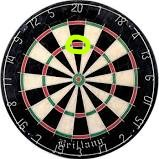
\includegraphics[scale=1.5]{Dartboard_colors.jpg}
	\caption{Dartboard with yellow circle around 60-point region}
\end{figure}

Assuming that all three darts could hit the dart board randomly, there is a finite (even though small) probability that all three will hit the triple score region (inner red-and-green ring) in the 20-point "slice" (see yellow circle in Fig.3.1). That would make each throw worth 60 points and therefore this would make a total possible score of 180 points for 3 throws. That would represent the highest possible score.\\
Now we design a Monte Carlo simulation for scoring three darts with the assumption of hitting the board at random and we list the scores of 5 sets of three-dart throws.
\[
\begin{bmatrix} 
      					Dart\#1 & Dart\#2 & Dart\#3 & Total \\
     					 16 & 8 & 25 & 49\\
					 1 & 14 & 0 & 15\\
					 25 & 0 & 15 & 40\\
					 0 & 11 & 0 & 11\\
					 0 & 9 & 12 & 21			  
\end{bmatrix}
\]

Thus, as we see, none of our random throws has given us the highest possible score. In fact, the highest score obtained in the simulation (49) is eleven points lower than the highest possible score that could be obtained by one throw in the triple region of the 20-point "slice."\\

\section{Part b}
Simulating the program 10,000 times give us the following mean value and standard deviation
$$
\mu = 34.1411
$$
$$
\sigma = 22.0310
$$
We can see that the mean value for 10,000 simulations is consistently different from what we would get by simply averaging the 5 sets of throws that we have obtained in Part a, in fact
$$
\frac{49+15+40+11+21}{5} = 27.2,
$$
which represents a value that is roughly 20\% smaller than the mean score obtained by simulating the program 10,000 times.

\section{Part c}

\begin{figure}[H]
	\centering
	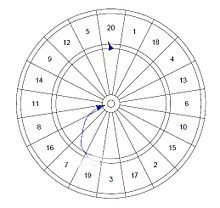
\includegraphics[scale=0.9]{Dartboard_optimal.jpg}
	\caption{Dartboard}
\end{figure}

Let's have a brief review of the most common rules followed in the game of darts.\\
The oche (line behind which the thrower must stand) should be 7 ft 9(1/2)in (2.37 m) from the face of the board.
Most games are usually played following the "501 up" rule. I.e. each player starts with 501 points and takes turns to throw 3 darts. The first player who reaches exactly 0 wins the game. It is a double out game, which means that players must hit a double that makes their score exactly zero to win the game. Moreover, if a player reduces the score to 1 or goes below to zero, the score is bust and his/her score is returned to that of his/her previous turn. If none of the players gets to zero in 20 turns, the player with the lower point wins.
If the scores are equal after 20 turns, the game will continue for another possible 10 turns.
During these extra turns, the player who gets to zero obviously wins. A player with lower score any time after the 20th turn also wins the match.
If the scores are equal after 20+10 turns, the match will end in a draw.\\
Thus, as we see, there are many variables that play into the game that have not been taken into account in our previous Monte Carlo simulation.\\
Assuming standard scoring, the optimal area to aim for on the dart board in order to maximise the player's score varies significantly based on the players' skill. The skilled player should aim for the centre of the T20 (the 20-point "slice") and as the player's skill decreases, their aim moves slightly up and to the left of the T20, according to $\textit{A Statistician Plays Darts}$, by R. Tibshirani, A. Price and J. Taylor.\\
So, we might want to modify our Monte Carlo Simulation by considering the players' different skill-sets and therefore their accuracy in their throws. For instance, we know from literature that for a player for perfect accuracy (practically extremely unlikely, but theoretically acceptable) the best place to aim is the center of the T20, whereas a player that throws randomly (amateur, first-time player) should aim into the centre of the dartboard, stopping a little lower and to the left of the bull's eye. So assuming that all players will try to maximise theirs scores in accordance to their different skills levels, we might want to run a simulation taking into account skill-sets, let's say having ability levels going from 1 to 10 (10 being the most-skilled), so that we could have a more realistic distribution of scores among players. For each throw, we might want to maximise the probability that each player will actually hit the section of the dartboard that he/she is aiming to, but we should also give a higher probability of that happening for better-skilled players and lower for not-so-skilled players.\\
So, for instance, let's assume that the most-skilled player (skill level 10) has a 96\% chance to hit the T20 for each throw. Then, the percentage of hitting the highest scoring region (the triple region) would be 20\% of the total chance for each throw, as there is less surface area to aim to, and same goes for the double region (as it has the same surface area of the triple region), and a 10\% chance to hit the bull's eye. Of the remaining 4\%, 99.9\% of chance to hit the regions next by and 0.1\% to not hit the dartboard or to hit the no-points region.\\
Let's give the least-skilled player (skill level 1) a 5\% probability to hit his desired target and a 50\% probability to hit the region of the dartboard that gives points (which means for every throw he has a 50\% chance to score zero points).\\
From these lower and upper limits we would build the conditions for all the remaining players (skill levels from 2 to 8). Then we would have to randomly extract, let's say, 5 players with different skill-sets and simulate a game among them.
Obviously there would be the necessity to take into account the fact that, as players either reach 1 point or go below zero, they bust and go back to the previous score. As best-skilled players would have a higher probability to win matches, they would also have a higher probability to find themselves in a critical situation with regard to their scores, which would require for them to change strategy in order to avoid busting.\\
These are some of the improvements that could be made to a have a more realistic simulation of a dartboard match.
%Now, to simplify our discussion, let's assume that the players are all professional or at least somewhat trained in the "sport" of darts, so that their skill-set is more or less uniform. So, all of them has trained himself/herself to get the most points from every single round, at least up until some arithmetic needs to be involved in order not to bust. So, most players will try to aim to the portion of the dartboard where they could get the most points, which is represented by the bull's eye (50 points worth of) straight up into the 20-point "slice", especially the triple and double region (which will be worth 60 and 40 points per throw respectively). Now, it is reasonable to assume that not all darts will end up in the desired spot, but, since the players are all well-trained, it is also reasonable to think that most of their darts will end up close to the desire spot. Let's say within 0.5 inches to their aim.%




\chapter{Problem 4}
We know that a stochastic birth only process could be represented by the following differential equation
$$
\frac{dP_{N}}{dt} + \lambda NP_{N} = \lambda (N-1)P_{N-1},
$$
with 
\[ 
P_{N}(0) =  
\begin{cases} 
      					0 & N\neq N_{0} \\
     					 1 & N =  N_{0} 
\end{cases}
\]

We know from lecture that 
$$
P_{N_{0}}(t) = e^{-\lambda}N_{0}t
$$
$$
P_{N_{0}+1}(t) = N_{0}e^{-\lambda N_{0}t}(1-e^{-\lambda t}),
$$ 
$$
\dots
$$
$$
P_{N_{0}+j}=\frac{N_{0}(N_{0}+1)\dots(N_{0}+j-1)}{j!}e^{-\lambda N_{0}t}(1-e^{-\lambda t})^{j}.
$$
we want to prove by induction that this holds for all possible $j$'s.
So, we know from literature that the relationship holds for $j=0,1$. Now, let's pick a $j_{0}$ such that $j \leq j_{0}$ and let's assume that the $P_{N_{0}+j}$ would hold for such values.
Using this assumption, we now have to prove that the statement holds for the next value $j_{0}+1$ and we will be done.\\
Thus, we have to determine $P_{N_{0}+j_{0}+1}$ using our differential equation with $N=N_{0}+j_{0}+1$. Using the formula for $P_{N_{0}+j_{0}}$, which is valid by our assumption, we get
$$
\frac{dP_{N_{0}+j_{0}+1}}{dt} + \lambda (N_{0}+j_{0}+1)P_{N_{0}+j_{0}+1} = \frac{N_{0}(N_{0}+1)\dots(N_{0}+j_{0})}{j_{0}!} e^{-\lambda N_{0} t} (1-e^{-\lambda t})^{j_{0}},
$$
where the initial condition is $P_{N_{0}+j_{0}+1}(0)=0$.\\
Here we show the various passages used to solve that derivative
\begin{align*}
\frac{dP_{N_0+j_{0}+1}(t)}{dt}&=\frac{N_0(N_0+1)\dots(N_0+j_{0})}{(j_{0}+1)!}\left((-\lambda N_0)e^{-\lambda N_0 t}(1-e^{-\lambda t})^{j_{0}+1}+e^{-\lambda N_0 t}(j_{0}+1)(1-e^{-\lambda t})^{j_{0}}(\lambda e^{-\lambda t})\right)\\
&=\frac{N_0(N_0+1)\dots(N_0+j_{0})}{(j_{0}+1)!}\left((- N_0)(1-e^{-\lambda t})+(j_{0}+1)(e^{-\lambda t})\right)\lambda(1-e^{-\lambda t})^{j_{0}}e^{-\lambda N_0 t}\\
&=\frac{N_0(N_0+1)\dots(N_0+j_{0})}{(j_{0}+1)!}\left(- N_0+N_0e^{-\lambda t}+e^{-\lambda t}+j_{0}e^{-\lambda t}\right)\lambda(1-e^{-\lambda t})^{j_{0}}e^{-\lambda N_0 t}\\
&=\frac{N_0(N_0+1)\dots(N_0+j_{0})}{(j_{0}+1)!}\left(- N_0+e^{-\lambda t}(N_0+j_{0}+1)\right)\lambda(1-e^{-\lambda t})^{j_{0}}e^{-\lambda N_0 t}\\
&= \frac{N_0(N_0+1)\dots(N_0+j_{0})}{(j_{0}+1)!}\left(-N_0-(j_{0}+1) +(N_0+j_{0}+1)e^{-\lambda t}+(j_{0}+1) \right)\lambda e^{-\lambda N_0 t}(1-e^{-\lambda t})^j_{0}\\
&= \frac{N_0(N_0+1)\dots(N_0+j_{0})}{(j_{0}+1)!}\left(-(N_0+j_{0}+1) (1-e^{-\lambda t})+(j_{0}+1) \right)\lambda e^{-\lambda N_0 t}(1-e^{-\lambda t})^j_{0}\\
&= - \lambda (N_0+j_{0}+1) \frac{N_0(N_0+1)\dots(N_0+j)}{(j_{0}+1)!}e^{-\lambda N_0 t}(1-e^{-\lambda t})^{j_{0}+1}+\\
&+\lambda (N_0+j_{0}) \frac{N_0(N_0+1)\dots(N_0+j_{0}-1)}{j_{0}!}e^{-\lambda N_0 t}(1-e^{-\lambda t})^{j_{0}}\\
&=\lambda (N_0+j_{0}) P_{N_0+j_{0}} - \lambda (N_0+j_{0}+1) P_{N_0+j_{0}+1}
\end{align*}
We can now compute the solution to this differential equation, which is found to be
$$
P_{N_{0}+j_{0}+1}=\frac{N_{0}(N_{0}+1)\dots(N_{0}+j_{0})}{(j_{0}+1)!}e^{-\lambda N_{0}t}(1-e^{-\lambda t})^{j_{0}+1}.
$$
Since we see that the formula holds for $j_{0}+1$ and, from our induction assumption, $j \leq j_{0}$ , then the formula holds for any value of $j$.
			

\chapter{Problem 5}
\section{Part a}
The expected population $E(t)$ at time $t$ is given by the formula
$$
E(t) = \sum_{j=0}^{\infty} (N_{0}+j)P_{N_{0}+j}(t),
$$
which holds for birth-only stochatics process. I.e. the population never decreases in size, so it can either increase or stay the same for some given interval of values of $j$. Thus, if we assume that our population can only be described by discrete integer numbers (as you cannot have "fractions" of individuals), then we can write the expected population at time $t$ as
$$
E(t) = \sum_{j=0}^{\infty}(j)P_{j}(t).
$$
Also, the initial value of the population cannot be zero, otherwise it will not produce offspring, and it obviously cannot be negative, as negative populations do not make physical sense. So the initial population has to have some value $N_{0} > 0$.\\
Therefore we have that $P_{j}(t) = 0$ for $j < N_{0}$. Thus, 
$$
E(t)=\sum_{j=0}^{\infty}(j)P_{j}(t)=\sum_{j=N_0}^{\infty}(j)P_{j}(t)=\sum_{j=0}^{\infty}(N_0+j)P_{N_0+j}(t).
$$
which is our formula for $E(t)$.

\section{Part b}
We want to show that $E(t)=N_0 e^{\lambda t}$. Therefore, let's take the derivative of $E(t)$ as defined in Part a:
\begin{align*}
\frac{dE(t)}{dt}&=\sum_{j=0}^{\infty}(N_0+j)\frac{dP_{N_0+j}(t)}{dt}\\
&=\sum_{j=0}^{\infty}(N_0+j)\left(-\lambda (N_0+j) P_{N_0+j} +\lambda (N_0+j-1) P_{N_0+j-1}\right)\\
&=\lambda \sum_{j=0}^{\infty}(N_0+j)\left(-(N_0+j) P_{N_0+j} + (N_0+j) P_{N_0+j-1}-P_{N_0+j-1}\right)\\
&=\lambda \sum_{j=0}^{\infty}\left(-(N_0+j)^2 P_{N_0+j} + (N_0+j)^2 P_{N_0+j-1}-(N_0+j)P_{N_0+j-1}\right)\\
&=\lambda \sum_{j=0}^{\infty}\left(-(N_0+j)^2 P_{N_0+j} + (N_0^2+(2j-1) N_0+j^2-j) P_{N_0+j-1}\right)\\
&=\lambda\left(N_0 P_{N_0}+(N_0+1) P_{N_0+1}+(N_0+2) P_{N_0+2}+\dots \right)\\
&= \lambda \sum_{j=0}^{\infty}(j)P_{j}(t)\\
&= \lambda E(t).
\end{align*}
Thus, we see that 
$$\frac{dE(t)}{dt}=\lambda E(t),
$$ 
whose unique solution is readily found to be $E(t)=N_0 e^{\lambda t}$. And we're done.

\section{Part c}
In Part b we have shown that
$$
E(t) = \sum_{j=0}^{\infty} (N_{0}+j)P_{N_{0}+j}(t) = N_{0}e^{\lambda t},
$$
which means that to compute an expected population $E(t)$ at time $t$, we do not need to solve an infinite sum, but simply evaluate a function for a given initial population. Moreover, this shows that the above infinite sum is just the solution of an non-autonomous first order differential equation (it has exactly the same form) whose constant is $N_{0}$.\\
More importantly, we can see that this model is simply the Malthusian growth model, where $N_{0}$ is just the starting population at $t=0$ and $\lambda$ is its growth rate. This is a well-known system that is readily analysed in all its properties. Therefore our study of the model is extremely simplified by our results obtained in Part b. 


\chapter{Problem 6}
From Problem 5b, we have
$$
E(t) = \sum_{j=0}^{\infty} (N_{0}+j)P_{N_{0}+j}(t) = N_{0}e^{\lambda t}
$$
We have $N_{0}=10,000$ and that the total number of births occurred in 20 days is 4,500.\\
So, assuming that no deaths will occur in this period since this is a birth-only stochastics process, we have that our expected population at $t=20$ is
$$
E(20) = 4,500 + 10,000 = 14,500.
$$
Therefore
$$
14,500 = 10,000e^{\lambda 20},
$$
from which we can easily solve for $\lambda$
$$
\lambda = \frac{\ln \left(\frac{14,500}{10,000}\right)}{20}
$$
from which we obtain
$$
\lambda \approx 0.0186
$$
Therefore the population has a growth rate of 1.86\%.

%\chapter{Problem 3}
%\input{Problem3_Latex}

%\chapter{Computational Application}
%\input{chapter4}





\end{document}
